% En esta seccion se presentan los resultados finales de los experimentos (versión final) mediante figuras y capturas de pantalla debidamente tituladas y referenciadas en el cuerpo del reporte. Analiza las ventajas y desventajas de la metodología aplicada.

\section{Resultados}

A continuación se presentan los resultados finales obtenidos en el desarrollo de la práctica, detallando el comportamiento cinemático del modelo articulado y el análisis de ventajas y desventajas de la metodología implementada.

\subsection{Actividad 1: Modelado de una pierna con articulaciones jerarquizadas en Blender}

Como resultado de esta primera actividad obtuvimos una pierna humana tridimensional, continua y anatómicamente articulada, capaz de flexionarse y deformarse de forma elástica mediante una armadura jerarquizada de cinco huesos. En la Tabla \ref{tab:resumen_huesos} se resumen las características de cada segmento esquelético, su dependencia en el árbol cinemático y su función anatómica. Al probar el modelo comprobamos que la cadena responde de manera completamente coherente a las transformaciones: al rotar la cadera en el origen, la extremidad completa se orienta y traslada en bloque; si giramos el fémur, la rodilla, el tobillo y los dedos acompañan la trayectoria conservando intacta su postura interna; al flexionar la tibia, únicamente se desplaza el pie respecto a la articulación de la rodilla; y al mover el metatarso, la rotación queda confinada exclusivamente al empeine y las falanges de los dedos.

\begin{table}[H]
\centering
\small
\begin{tabular}{@{}cp{3.4cm}p{3.4cm}p{2.6cm}p{5.0cm}@{}}
\toprule
\textbf{\#} & \textbf{Nombre del hueso} & \textbf{Hueso padre} & \textbf{Conexión} & \textbf{Función anatómica} \\
\midrule
1 & \texttt{1\_Cadera\_Pelvis}   & \textit{Ninguno (Raíz)} & Raíz (libre)       & Pivote base superior de la cadera. \\
2 & \texttt{2\_Muslo\_Femur}     & \texttt{1\_Cadera\_Pelvis}   & \texttt{Connected} & Flexión y rotación del muslo. \\
3 & \texttt{3\_Espinilla\_Tibia} & \texttt{2\_Muslo\_Femur}     & \texttt{Connected} & Flexión de la rodilla. \\
4 & \texttt{4\_Pie\_Metatarso}   & \texttt{3\_Espinilla\_Tibia} & \texttt{Connected} & Flexión del tobillo y pie. \\
5 & \texttt{5\_Dedos\_Pie}       & \texttt{4\_Pie\_Metatarso}   & \texttt{Connected} & Apoyo y despegue de falanges. \\
\bottomrule
\end{tabular}
\caption{Estructura jerárquica de la armadura desarrollada en Blender para la Actividad 1.}
\label{tab:resumen_huesos}
\end{table}

En la Figura \ref{fig:resultado_pierna} se compara el estado final de la pierna en su pose neutral de reposo (\textit{Rest Pose}, izquierda) frente a una postura de flexión articular en Modo Pose (derecha). Como se puede apreciar en las capturas, la combinación del sombreado suave con el modificador de Subdivisión de Superficie en nivel 2 y la dispersión subsuperficial produce una silueta orgánica limpia y sin facetas poligonales visibles. Lo más destacable del resultado visual es que la masa muscular del cuádriceps, la prominencia de la rótula y la curvatura de los gemelos se conservan de forma convincente durante el movimiento, demostrando que los bucles cuadriláteros que añadimos en el modelado cumplieron su propósito de evitar el colapso de la geometría.

\begin{figure}[H]
    \centering
    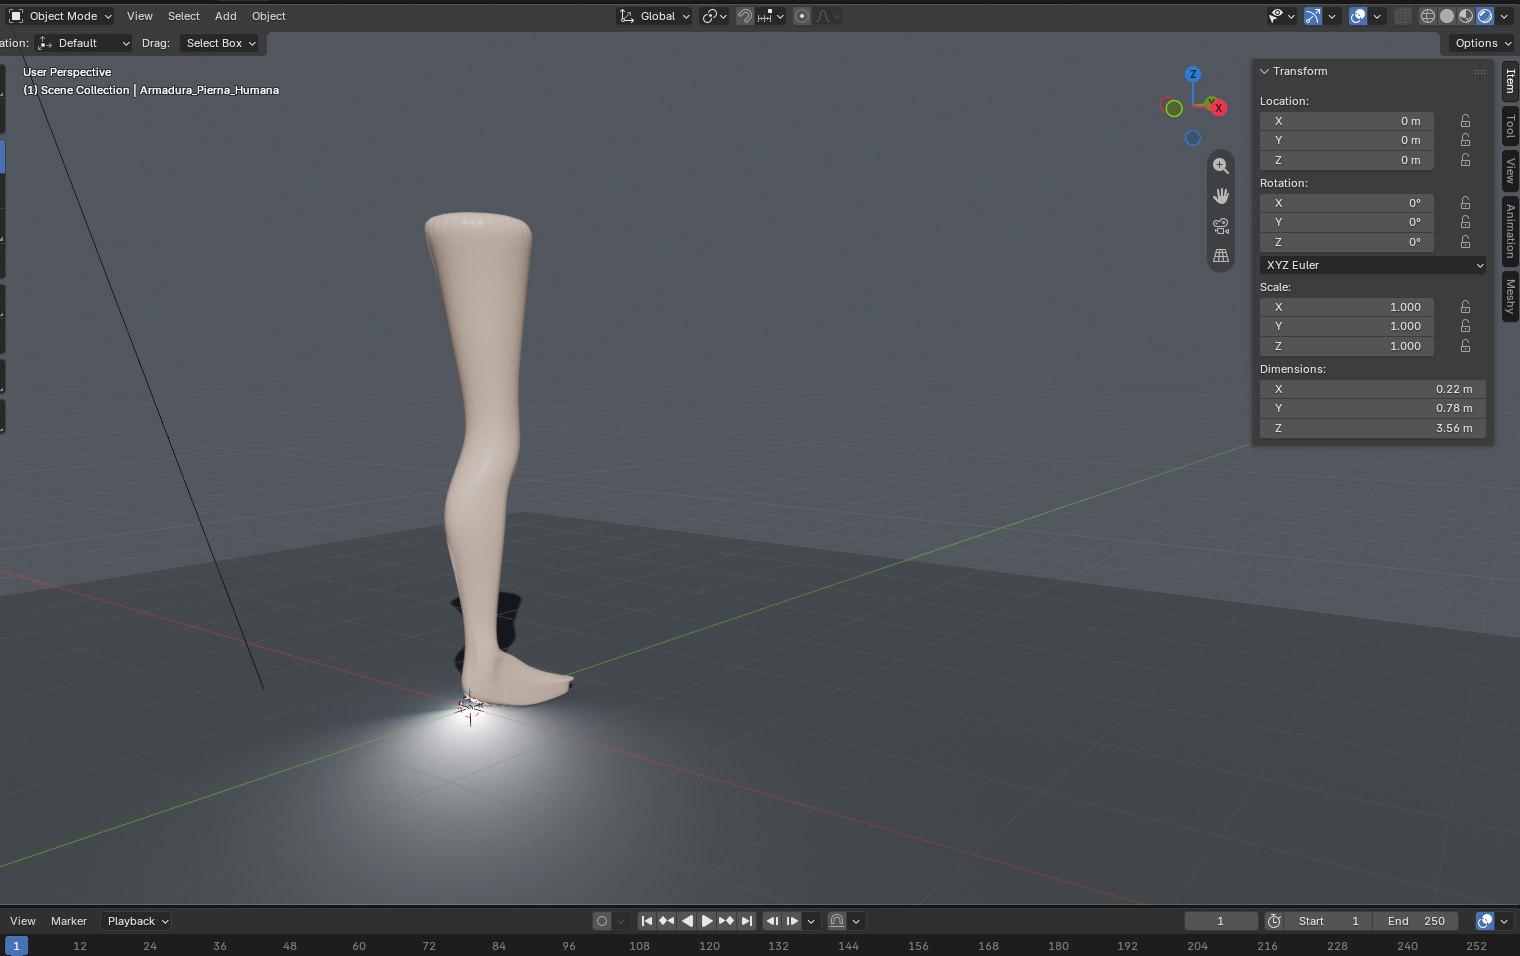
\includegraphics[width=0.45\textwidth]{Imagenes/E1/03_pierna_pose_reposo.png}
    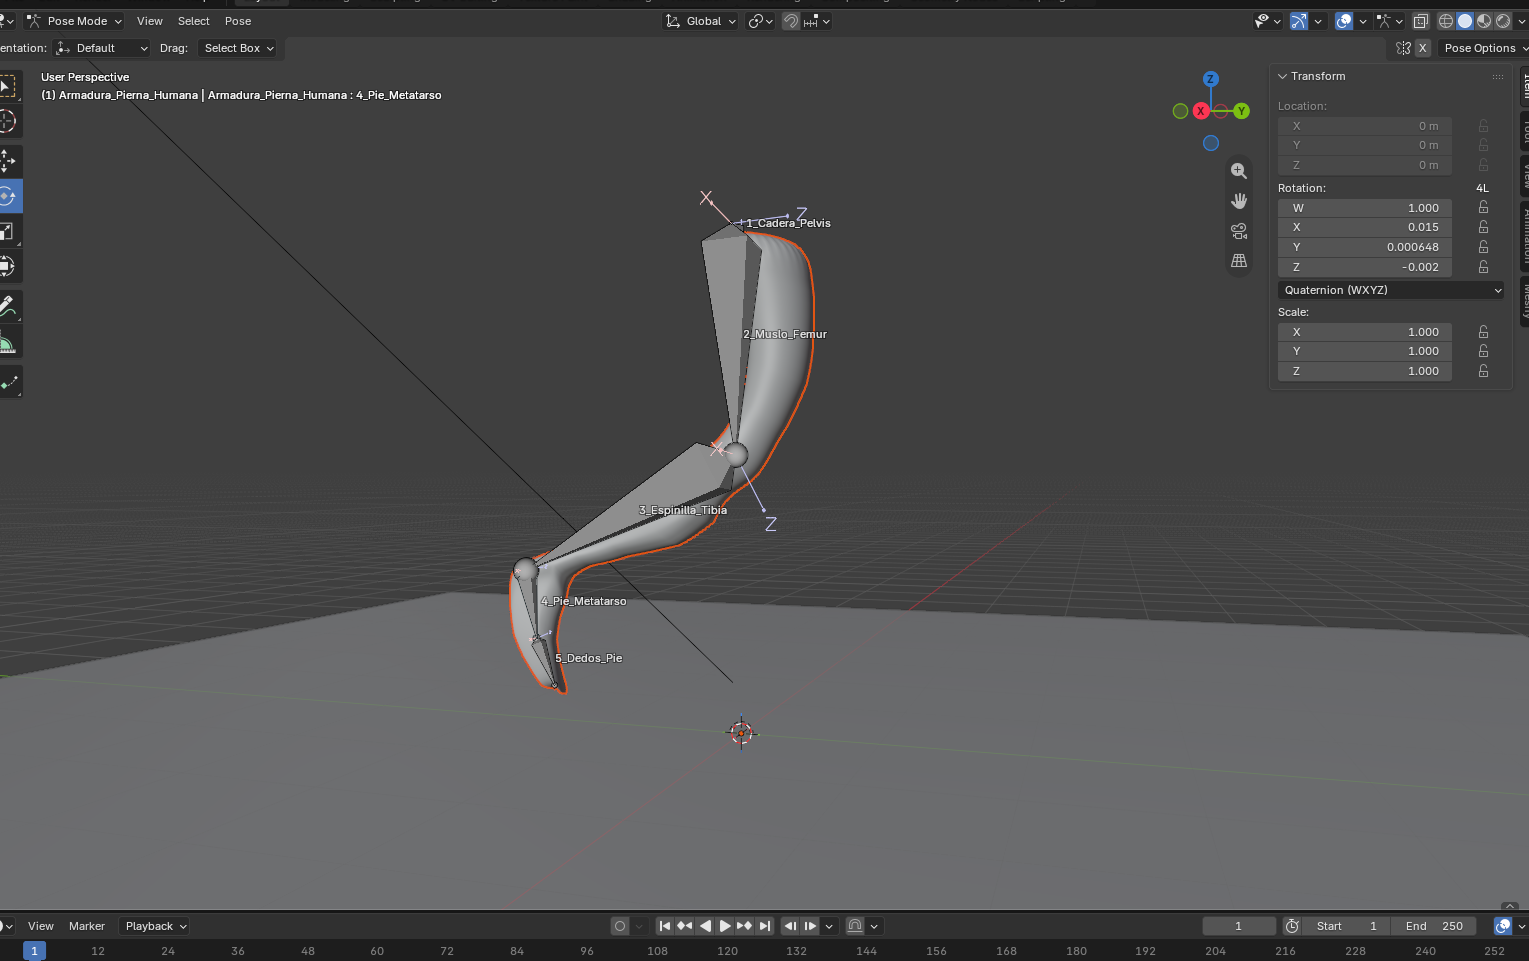
\includegraphics[width=0.45\textwidth]{Imagenes/E1/04_demostracion_fk_flexion_rodilla.png}
    \caption{Resultado final de la Actividad 1: a la izquierda, modelo completo de la pierna en pose neutral de reposo (\textit{Rest Pose}); a la derecha, demostración en Modo Pose flexionando rodilla y tobillo mediante cinemática directa (FK).}
    \label{fig:resultado_pierna}
\end{figure}

Al evaluar las ventajas de la metodología que seguimos, la principal fortaleza estuvo en haber modelado la pierna como una sola pieza continua en lugar de ensamblar cilindros y cajas independientes. Esto no solo le da un acabado mucho más realista a la piel, sino que permitió que el algoritmo de difusión de calor de Blender (\textit{Automatic Weights}) calculara degradados de peso continuos y suaves, ahorrándonos el trabajo de tener que pintar la influencia de cada vértice de forma manual. Igualmente, configurar los huesos con la propiedad \texttt{Connected} nos garantizó que las articulaciones mantuvieran siempre el contacto en los pivotes, evitando cualquier desprendimiento accidental de las extremidades al rotarlas. Desde el punto de vista didáctico, trabajar con Cinemática Directa (FK) nos resultó muy formativo para entender en la práctica cómo opera la propagación jerárquica de matrices ($M_{\text{global}} = M_{\text{padre}} \cdot M_{\text{local}}$), ya que pudimos inspeccionar de primera mano cómo cada transformación local afecta en cascada a todos sus descendientes.

En cuanto a las desventajas y limitaciones que identificamos, la más evidente es la dificultad que presenta la Cinemática Directa cuando se intenta animar una interacción de contacto fijo con el suelo. Para simular que la planta del pie se queda apoyada mientras el cuerpo avanza, con FK es necesario reajustar manualmente la cadera, el muslo, la pantorrilla y el metatarso en cada fotograma, lo cual se vuelve muy tedioso y poco preciso en comparación con un sistema de Cinemática Inversa (IK), donde bastaría con arrastrar el pie a su posición deseada y dejar que la rodilla se flexione de forma automática. Por otro lado, aunque el modificador de subdivisión deja la superficie impecable para renderizado estático o ilustración, el conteo de polígonos resultante es demasiado alto para una aplicación gráfica interactiva o un motor en tiempo real como OpenGL, lo que en un flujo de trabajo profesional obligaría a realizar una retopología o a hornear las normales sobre una malla de baja resolución. Finalmente, notamos que si bien los pesos automáticos retienen bien el volumen en rangos normales de flexión (hasta unos $90^\circ$), en flexiones muy cerradas que superan los $120^\circ$ se aprecia un leve aplanamiento en el pliegue poplíteo posterior, un detalle que en una producción avanzada requeriría apoyarse en claves de forma correctivas (\textit{Corrective Shape Keys}) para mantener la masa muscular intacta.

\subsection{Actividad 2: Animación y análisis de relaciones padre-hijo de un personaje de Adobe Mixamo en Blender}
% [Pendiente de desarrollo]

\subsection{Actividad 3: Diagrama de las relaciones padre-hijo de la estructura jerárquica desde el nodo raíz}
% [Pendiente de desarrollo]

\subsection{Actividad 4: Exploración de software para estructuras humanoides (MakeHuman y DAZ3D)}
% [Pendiente de desarrollo]